% BEGIN GENERATED:pathway_figure
% generator: cdrt.report 1 (pathway_figure)
% inputs: capture/bundle/BUNDLE.json 1bd0e42b0dff
% lock_root: 5027e2dd7806fc031b01e5880fcd83a8cca3381d7eb3cc3d5be6e4f1d233387c  campaign: campaign-002
% commit: 94766191d437ffb3b094db957e369b9e98784e51
\begin{figure*}[pos=t]
\centering
% generator: cdrt.report 1 (figures/pathways.tex); lock_root: 5027e2dd7806fc031b01e5880fcd83a8cca3381d7eb3cc3d5be6e4f1d233387c; commit: 94766191d437ffb3b094db957e369b9e98784e51
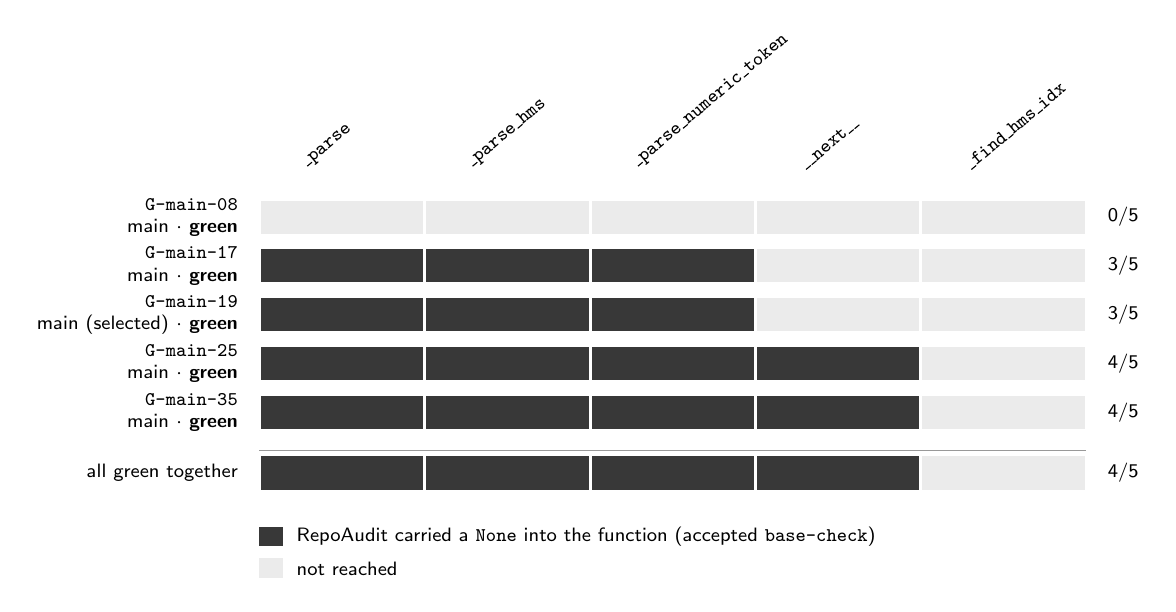
\begin{tikzpicture}[x=1cm,y=1cm,font=\sffamily\scriptsize]
\node[anchor=south west,rotate=40,inner sep=1pt] at (0.630,0.12) {\texttt{\_parse}};
\node[anchor=south west,rotate=40,inner sep=1pt] at (2.730,0.12) {\texttt{\_parse\_hms}};
\node[anchor=south west,rotate=40,inner sep=1pt] at (4.830,0.12) {\texttt{\_parse\_numeric\_token}};
\node[anchor=south west,rotate=40,inner sep=1pt] at (6.930,0.12) {\texttt{\_\_next\_\_}};
\node[anchor=south west,rotate=40,inner sep=1pt] at (9.030,0.12) {\texttt{\_find\_hms\_idx}};
\node[anchor=east,align=right] at (-0.15,-0.410) {\texttt{G-main-08}\\main $\cdot$ \textbf{green}};
\fill[black!8] (0.020,-0.620) rectangle ++(2.060,0.420);
\fill[black!8] (2.120,-0.620) rectangle ++(2.060,0.420);
\fill[black!8] (4.220,-0.620) rectangle ++(2.060,0.420);
\fill[black!8] (6.320,-0.620) rectangle ++(2.060,0.420);
\fill[black!8] (8.420,-0.620) rectangle ++(2.060,0.420);
\node[anchor=west] at (10.650,-0.410) {0/5};
\node[anchor=east,align=right] at (-0.15,-1.030) {\texttt{G-main-17}\\main $\cdot$ \textbf{green}};
\fill[black!78] (0.020,-1.240) rectangle ++(2.060,0.420);
\fill[black!78] (2.120,-1.240) rectangle ++(2.060,0.420);
\fill[black!78] (4.220,-1.240) rectangle ++(2.060,0.420);
\fill[black!8] (6.320,-1.240) rectangle ++(2.060,0.420);
\fill[black!8] (8.420,-1.240) rectangle ++(2.060,0.420);
\node[anchor=west] at (10.650,-1.030) {3/5};
\node[anchor=east,align=right] at (-0.15,-1.650) {\texttt{G-main-19}\\main (selected) $\cdot$ \textbf{green}};
\fill[black!78] (0.020,-1.860) rectangle ++(2.060,0.420);
\fill[black!78] (2.120,-1.860) rectangle ++(2.060,0.420);
\fill[black!78] (4.220,-1.860) rectangle ++(2.060,0.420);
\fill[black!8] (6.320,-1.860) rectangle ++(2.060,0.420);
\fill[black!8] (8.420,-1.860) rectangle ++(2.060,0.420);
\node[anchor=west] at (10.650,-1.650) {3/5};
\node[anchor=east,align=right] at (-0.15,-2.270) {\texttt{G-main-25}\\main $\cdot$ \textbf{green}};
\fill[black!78] (0.020,-2.480) rectangle ++(2.060,0.420);
\fill[black!78] (2.120,-2.480) rectangle ++(2.060,0.420);
\fill[black!78] (4.220,-2.480) rectangle ++(2.060,0.420);
\fill[black!78] (6.320,-2.480) rectangle ++(2.060,0.420);
\fill[black!8] (8.420,-2.480) rectangle ++(2.060,0.420);
\node[anchor=west] at (10.650,-2.270) {4/5};
\node[anchor=east,align=right] at (-0.15,-2.890) {\texttt{G-main-35}\\main $\cdot$ \textbf{green}};
\fill[black!78] (0.020,-3.100) rectangle ++(2.060,0.420);
\fill[black!78] (2.120,-3.100) rectangle ++(2.060,0.420);
\fill[black!78] (4.220,-3.100) rectangle ++(2.060,0.420);
\fill[black!78] (6.320,-3.100) rectangle ++(2.060,0.420);
\fill[black!8] (8.420,-3.100) rectangle ++(2.060,0.420);
\node[anchor=west] at (10.650,-2.890) {4/5};
\draw[black!40] (0,-3.370) -- (10.500,-3.370);
\node[anchor=east,align=right] at (-0.15,-3.660) {all green together};
\fill[black!78] (0.020,-3.870) rectangle ++(2.060,0.420);
\fill[black!78] (2.120,-3.870) rectangle ++(2.060,0.420);
\fill[black!78] (4.220,-3.870) rectangle ++(2.060,0.420);
\fill[black!78] (6.320,-3.870) rectangle ++(2.060,0.420);
\fill[black!8] (8.420,-3.870) rectangle ++(2.060,0.420);
\node[anchor=west] at (10.650,-3.660) {4/5};
\fill[black!78] (0,-4.590) rectangle ++(0.3,0.25);
\node[anchor=west] at (0.35,-4.470) {RepoAudit carried a \texttt{None} into the function (accepted \texttt{base-check})};
\fill[black!8] (0,-4.990) rectangle ++(0.3,0.25);
\node[anchor=west] at (0.35,-4.870) {not reached};
\end{tikzpicture}

\caption{Same green, different paths. Each row is one green decision captured from RepoAudit, with the same model, target and question; each column is a function in the auditor's scope $M_h$, ordered by how many runs reached it. A dark cell means the run carried a \texttt{None} into that function, which is what an accepted \texttt{base-check} requires. The verdicts are identical; the checking behind them is not. \PathwaySentence{}}
\label{fig:pathways}
\end{figure*}
% END GENERATED:pathway_figure
